\section{Overall description}
The purpose of this section is to provide a brief description of the project and to describe known actors and their interaction with the system. The section presents a high level view. For more detailed information, please refer to the developer team.

	\subsection{Stakeholders}
	\begin{itemize}
		\item \textbf{Rowing club administrators:} Must integrate the system into the rowing club's network infrastructure. Their concern is, that the system is usable for logging routes without any extended knowledge of computer systems.
		\item \textbf{Developers:} JEE course students, that are developing the system. Developers include architects, testers and quality engineers.
		\item \textbf{Rowing club members:} Use the system to log their rowed routes.
		\item \textbf{Lecturer:} Checks the state of development and marks the result of the developers for the JEE course.
		\item \textbf{Rowing club:} Organization that profits from the system, because it offers the possibility to create detailed statistics and provides a log.
		\item \textbf{Insurance company:} Interested in accident cases to view logged routes.
	\end{itemize}
	
	\subsection{Actors}
	The following actors can be defined:\\
	
	\begin{itemize}
		\item \textbf{Rowing club administrator:} The rowing club administrator uses the system to create and publish boats and routes. Rowing club administrators also use the system to generate analysis and view statistics. Another task of him is to observe the status of boats for retrieving information about damaged boats.
		\item \textbf{Rowing club member:} The rowing club member uses the system to log their rowed routes and publish these routes on their profile.
	\end{itemize}
	
	
	\subsection{Use case Model Survey}
	According to the six parts identified in section \ref{scope}, the use case model is broken into packages. The use cases presented in this survey are high level use cases and are presented in figure \ref{img:rowbuddyPackages}.
	
	\begin{figure}[H]
		\begin{center}
			\includegraphics[width=0.5\textwidth]{./figures/RowBuddy_packages.pdf}
			\caption{RowBuddy Packages}
			\label{img:rowbuddyPackages}
		\end{center}
	\end{figure}

		\subsubsection{Package RowBuddy Boat Management}

		\begin{figure}[H]
			\begin{center}
				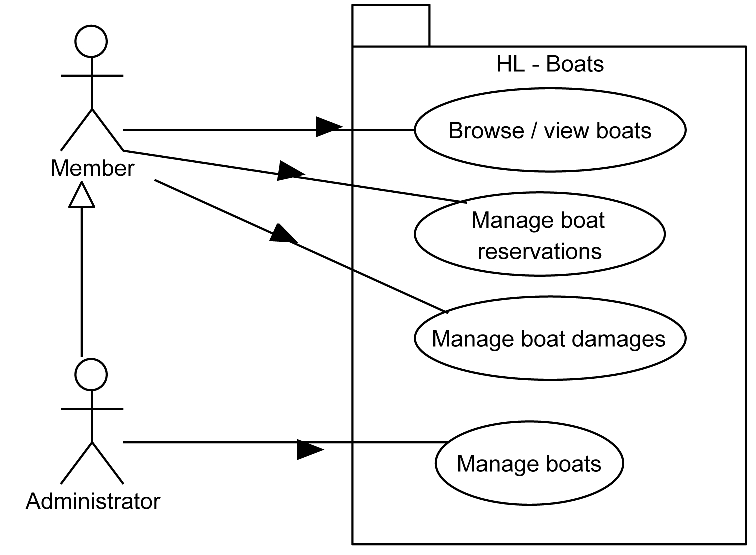
\includegraphics[width=0.6\textwidth]{./figures/HL-BoatManagement.pdf}
				\caption{Use case diagram package boat management}
				\label{img:UCBoatManagement}
			\end{center}
		\end{figure}

		\hluc{HLUC-1}{Browse / view boats}{Boats}{1}{gef}{}{%
A member can browse through the boats that exist in the system and view the details of a boat. The detail view of a boat contains information about the properties of a boat like the number of rowers and information about if the boat has a cox.}

		\hluc{HLUC-2}{Manage boats}{Boats}{1}{gef}{}{%
An administrator can add, edit and delete boats in the system. A boat that is deleted is completely removed from the system as long as it is not used in any other part of the system. If it is deleted and still referenced anywhere, it is visible in any parts where it is referenced, but it cannot be selected any longer for boat relevant actions. A boat can be locked and unlocked so that it cannot be used for trips if it is broken or under repair. }

		\hluc{HLUC-3}{Manage boat reservations}{Boats}{1}{gef}{}{%
If a member wants to use certain boats at a certain point in the future he is able to reserve them. Therefore he can select a time period and boats that are available during that time. If boats are blocked by other reservations he is able to see that, too. A reservation can be modified or deleted by the person that has created it and an administrator. Modification includes the adding and removing of additional boats. During reservation time the reserved boats can only be used by the person that has reserved the boat. }

		\hluc{HLUC-4}{Manage boat damages}{Boats}{1}{gef}{}{%
A member can record a damage that has occurred on a boat. He browses for a boat and chooses to add a damage. He enters information about the damage on the boat and additional information on the circumstances how the damage has happened. The creator and an administrator is able to edit the damage. An administrator can resolve the damage as fixed. A damage that is not fixed yet does not block a boat for trips. 
}

		\subsubsection{Package RowBuddy Member Management}

		\begin{figure}[H]
			\begin{center}
				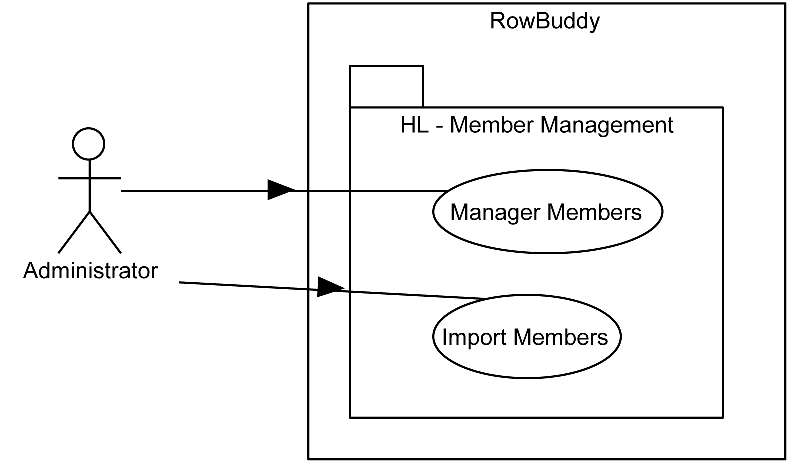
\includegraphics[width=0.6\textwidth]{./figures/HL-MemberManagement.pdf}
				\caption{Use case diagram package member management}
				\label{img:UCMemberManagement}
			\end{center}
		\end{figure}

		\hluc{HLUC-5}{Manage Members}{Member Management}{1}{gef}{}{%
An administrator can manage the members in the system. The information that is stored for a member is his address and the email address. A member can be marked as inactive. His data is still appearing in all statistical reports. A member can have certain roles. Every member has the role \emph{member}, optionally he can have the role \emph{administrator}. }

		\hluc{HLUC-6}{Import Members}{Member Management}{1}{gef}{}{%
An administrator can import members from a table based file. This is used to import a large amount of member data. A member is identified by its member-id. If a member-id does already exist in the system, all member data is overridden with the imported data.
}
		\subsubsection{Package RowBuddy Member Profiles}

		\begin{figure}[H]
			\begin{center}
				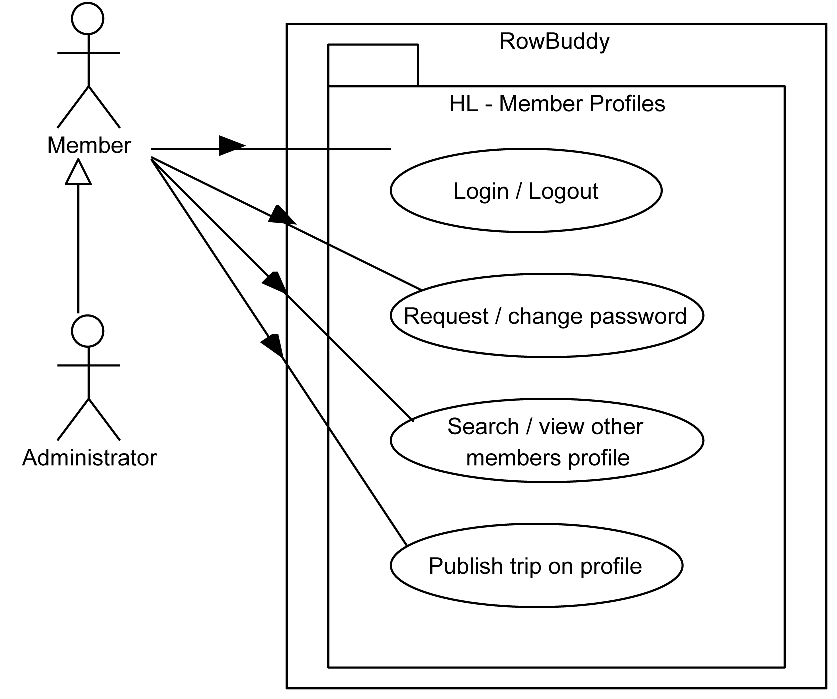
\includegraphics[width=0.6\textwidth]{./figures/HL-MemberProfiles.pdf}
				\caption{Use case diagram package member profiles}
				\label{img:UCMemberProfiles}
			\end{center}
		\end{figure}

		\hluc{HLUC-7}{Login / Logout}{Member Profiles}{1}{hei}{}{%
The user enters the email address that is known to the club and a password to authenticate himself regarding the system. After a successful login the user is able to view user-specific pages. A user that is not authenticated is only able to view an info page that shows whom he has to contact to get a user account. If the user does not visit any other pages for 1 hour, or clicked on logout, the user is logged out of the system.
}

		\hluc{HLUC-8}{Request / change password}{Member Profiles}{1}{hei}{}{%
The user can change his password. For that he has to be logged into the system. He enters his current password and the new password twice. The old password can not be used any more for a login, the new password is valid now.
If a user has not logged in into the system at all, he is able to request a temporary password by providing his e-mail address, which is used to mail the password. The users e-mail address has to be known to the system before the password can be requested. If the user has forgotten his password he can also request it. In this case an e-mail is dispatched with a link to confirm that he really wants to change his password. If the confirmation is done, a new e-mail is sent with his new temporary password. The temporary password should be changed afterwards.
}

		\hluc{HLUC-9}{Search / view other members profile}{Member Profiles}{1}{hei}{}{%
A users profile can be searched for when a user is logged in. The user is able to provide keywords for a full-text-search, or use a name, e-mail-address, role type or member since field to conduct the search.
Logged in users can view other users profiles. The information shown on a profile includes the name, surname, birth date, e-mail-address, roles, published trips, since when the user is member of the club and if the user is active.
}

		\hluc{HLUC-10}{Publish trip on profile}{Member Profiles}{1}{hei}{}{%
A user can publish selected trips on his profile. These trips can be selected as published in a users personal rowed routes view. After a user has checked a trip as published other users can view it under a users published trip site on his profile.
}

		\subsubsection{Package RowBuddy Route Management}

		\begin{figure}[H]
			\begin{center}
				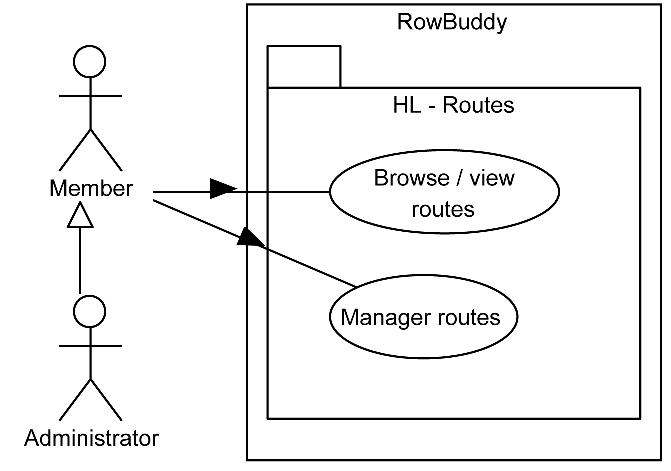
\includegraphics[width=0.6\textwidth]{./figures/HL-Routes.pdf}
				\caption{Use case diagram package routes}
				\label{img:UCRoutes}
			\end{center}
		\end{figure}

		\hluc{HLUC-11}{Browse / view routes}{Routes}{1}{gef}{}{%
A member is able to browse all routes in the system. He can view all details concerning a route. These are a description, the length and a map showing the points of the route. }

		\hluc{HLUC-12}{Manage routes}{Routes}{1}{gef}{}{%
A member can add, edit and delete routes in the system. Routes can be edited and deleted by any member if they are marked as mutable. Otherwise they can only be edited and deleted by the owner and administrators. If a route is modified the trips that have already used this route must not be altered, otherwise the log book would be manipulated. Therefore, edited routes exist as a new version of the route. If the current version of the route is not used yet, no new version has to be created.}

		\subsubsection{Package RowBuddy Statistics}

		\begin{figure}[H]
			\begin{center}
				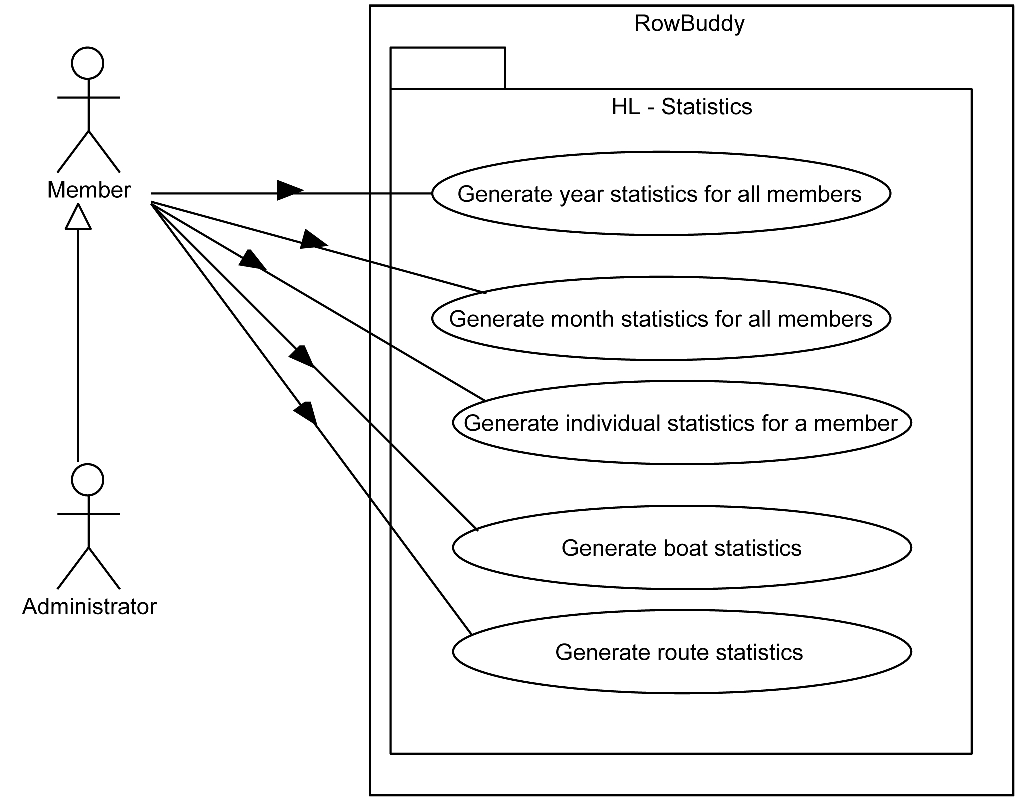
\includegraphics[width=0.6\textwidth]{./figures/HL-Statistics.pdf}
				\caption{Use case diagram package statistics}
				\label{img:UCStatistics}
			\end{center}
		\end{figure}

		\hluc{HLUC-13}{Generate year statistics for all members}{Statistics}{1}{hei}{}{%
Users can watch year statistics for all members, including a high score statistic that shows how many km a user has rowed in total over a year.
}

		\hluc{HLUC-14}{Generate month statistics for all members}{Statistics}{1}{hei}{}{%
Users can watch a statistic for all members that shows a high score of how many km a user has rowed in total over a month. Additionally a monthly activity statistic is available.
}

		\hluc{HLUC-15}{Generate individual statistics for a member}{Statistics}{1}{hei}{}{%
Individual statistics are generated on demand that can only be watched by the member that owns the particular statistic. These statistics include a year and month statistic that show how many km a user has rowed in a specific boat combined with the date.
}

		\hluc{HLUC-16}{Generate boat statistics}{Statistics}{1}{hei}{}{%
Boat statistics are generated on demand that show a high score list of the rowed km of each boat. Additionally a damaged boat statistic for a year can be viewed.
}

		\hluc{HLUC-17}{Generate route statistics}{Statistics}{1}{hei}{}{%
A year statistic of the most popular routes can be viewed by the users. It shows how often a specific route has been chosen for a tour in form of a high score list.
}

		\subsubsection{Package RowBuddy Trips}

		\begin{figure}[H]
			\begin{center}
				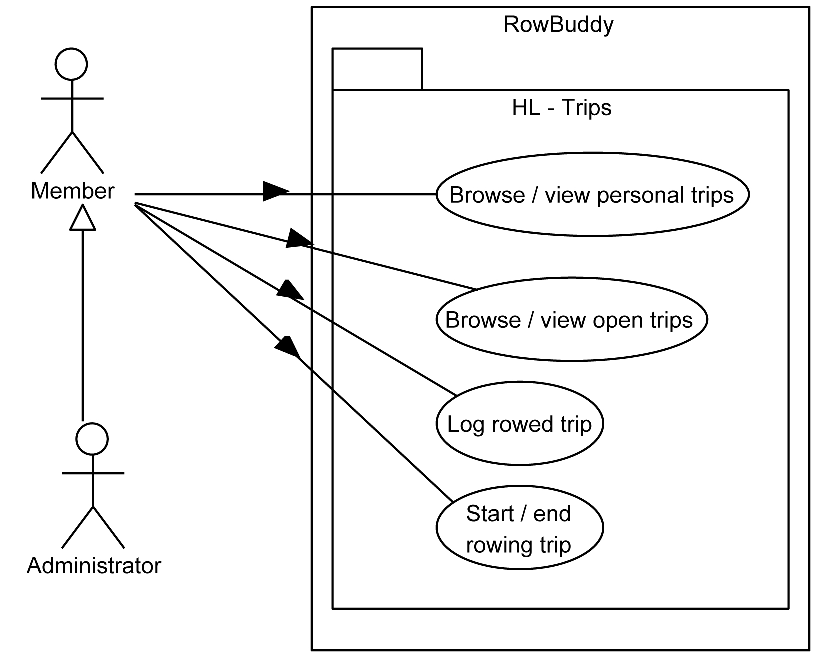
\includegraphics[width=0.6\textwidth]{./figures/HL-Trips.pdf}
				\caption{Use case diagram package trips}
				\label{img:UCTrips}
			\end{center}
		\end{figure}

		\hluc{HLUC-18}{Browse / view personal trips}{Trips}{1}{hei}{}{%
A user can browse through his personal trips taken. The browse list gives a short overview consisting of the route name, the ending- and starting-date and how many members attended the trip. The trips can be looked at in detail, with information such as the member names, the cox, the name of the boat and additional information about the trip.
This view is available for open and finished trips.
}

		\hluc{HLUC-19}{Browse / view open trips}{Trips}{1}{hei}{}{%
A user can browse through all currently open trips. The browse list gives a short overview consisting of the route name, the ending- and starting-date and how many members attended the trip. The trips can be looked at in detail, with information such as the member names, the cox, the name of the boat and additional information about the trip. In the detail view an open trip can be ended.
}

		\hluc{HLUC-20}{Log rowed trip}{Trips}{1}{hei}{}{%
A user can log an already rowed trip. The information that can be entered is start-date, end-date, the route (the user is able to search for existing routes), the members of the trip (existing members can be searched), the boat (existing boats can be searched as well) and additional information about the trip.
}

		\hluc{HLUC-21}{Start / end rowing trip}{Trips}{1}{hei}{}{%
A user can start a trip. The information that be entered is the same as in HLUC-20, except for the start-date (which is automatically set then) and the end-date, which is open.
The trip can then be ended in the open trips-overview detail-view. (HLUC-19) 
}

\subsection{Domain Model}
The following figure \ref{img:DomainModel} shows the domain model of the RowBuddy system.

		\begin{figure}[H]
			\begin{center}
				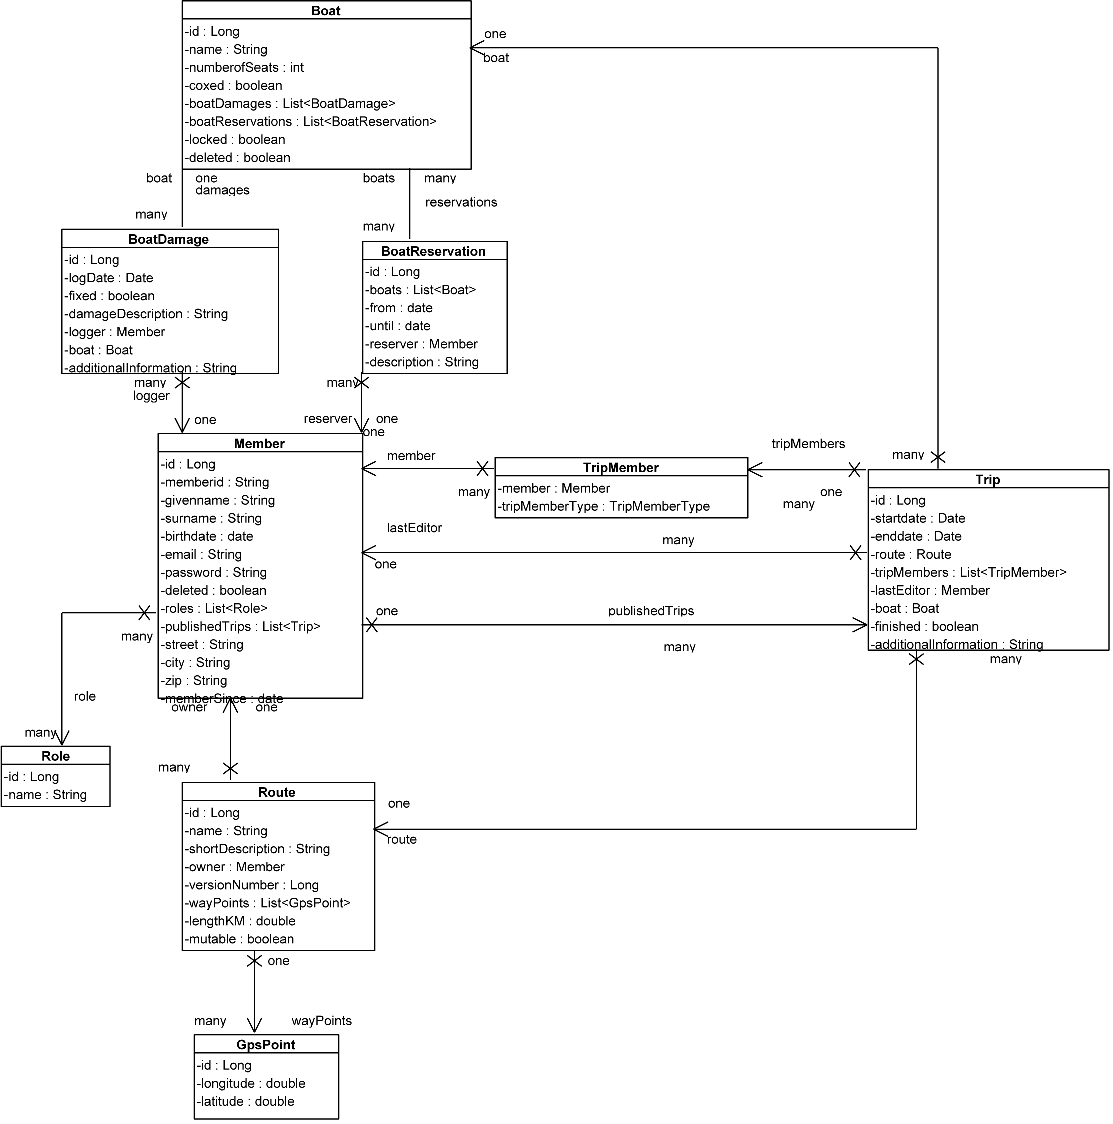
\includegraphics[width=1.0\textwidth]{./figures/DomainModel.pdf}
				\caption{RowBuddy Domain Model}
				\label{img:DomainModel}
			\end{center}
		\end{figure}




		